\chapter{Resultados e Discussão}\label{chapter:resultados_e_discussoes}

Para discussão dos resultados obtidos, deve-se retomar os objetivos propostos na \autoref{section:objetivos}. Alcançar os objetivos funcionais do projeto está condicionado à escolha de um \textit{hardware} que atenda todos os itens definidos como requisito. Dessa forma, o dispositivo escolhido para a prototipagem (B-L475E-IOT01A2) atendeu todos os requisitos funcionais do projeto, assim como os requisitos mínimos recomendados pela AWS. Esse dispositivo atende também os requisitos não-funcionais estipulados, uma vez que ele é qualificado pela AWS, apresenta versatilidade (contando com vários sensores, Bluetooth, Wi-Fi, sensor NFC, suporte à conexões em baixas frequências e microfones) e possui um preço de mercado inferior a seus concorrentes, uma vez que apresenta configurações mínimas para o desenvolvimento de aplicações AWS.

Durante os testes com o dispositivo, a empresa STMicroelectronics ofereceu suporte em seus canais de comunicação, o que acelerou o processo de prototipagem. Em contraponto, muitos códigos de exemplo fornecidos pela mesma empresa continham problemas de configuração de compilação, o que atrasou e dificultou o processo de desenvolvimento. Ademais, o processo de importação de produtos para prototipagem, assim como de outros produtos eletrônicos para o Brasil, possui alta alíquota de imposto, podendo chegar a 95\% do FOB (valor da mercadoria e outras despesas anteriores ao embarque), o que encareceu o projeto.

Para a validação da habilidade \textit{B-L475E-IOT01A2-Skill}, fez-se uso do \textit{Amazon Alexa Console} e do \textit{Cliente de teste MQTT}. Ao pronunciar a frase ``set led on'' para a Alexa, é possível visualizar que uma mensagem de mudança de estado do LED é recebida no tópico ``\$aws/things/B-L475E-IOT01A2/shadow/update''. As figuras \autoref{fig:alexa_developer_console} e \autoref{fig:cliente_de_teste_mqtt} mostram capturas de tala do processo de validação da habilidade \textit{B-L475E-IOT01A2-Skill}.

\begin{figure}[htbp]
	\centering
	\caption{Simulação de uma iteração do usuário com a Alexa através do \textit{Amazon Alexa Console}.}
	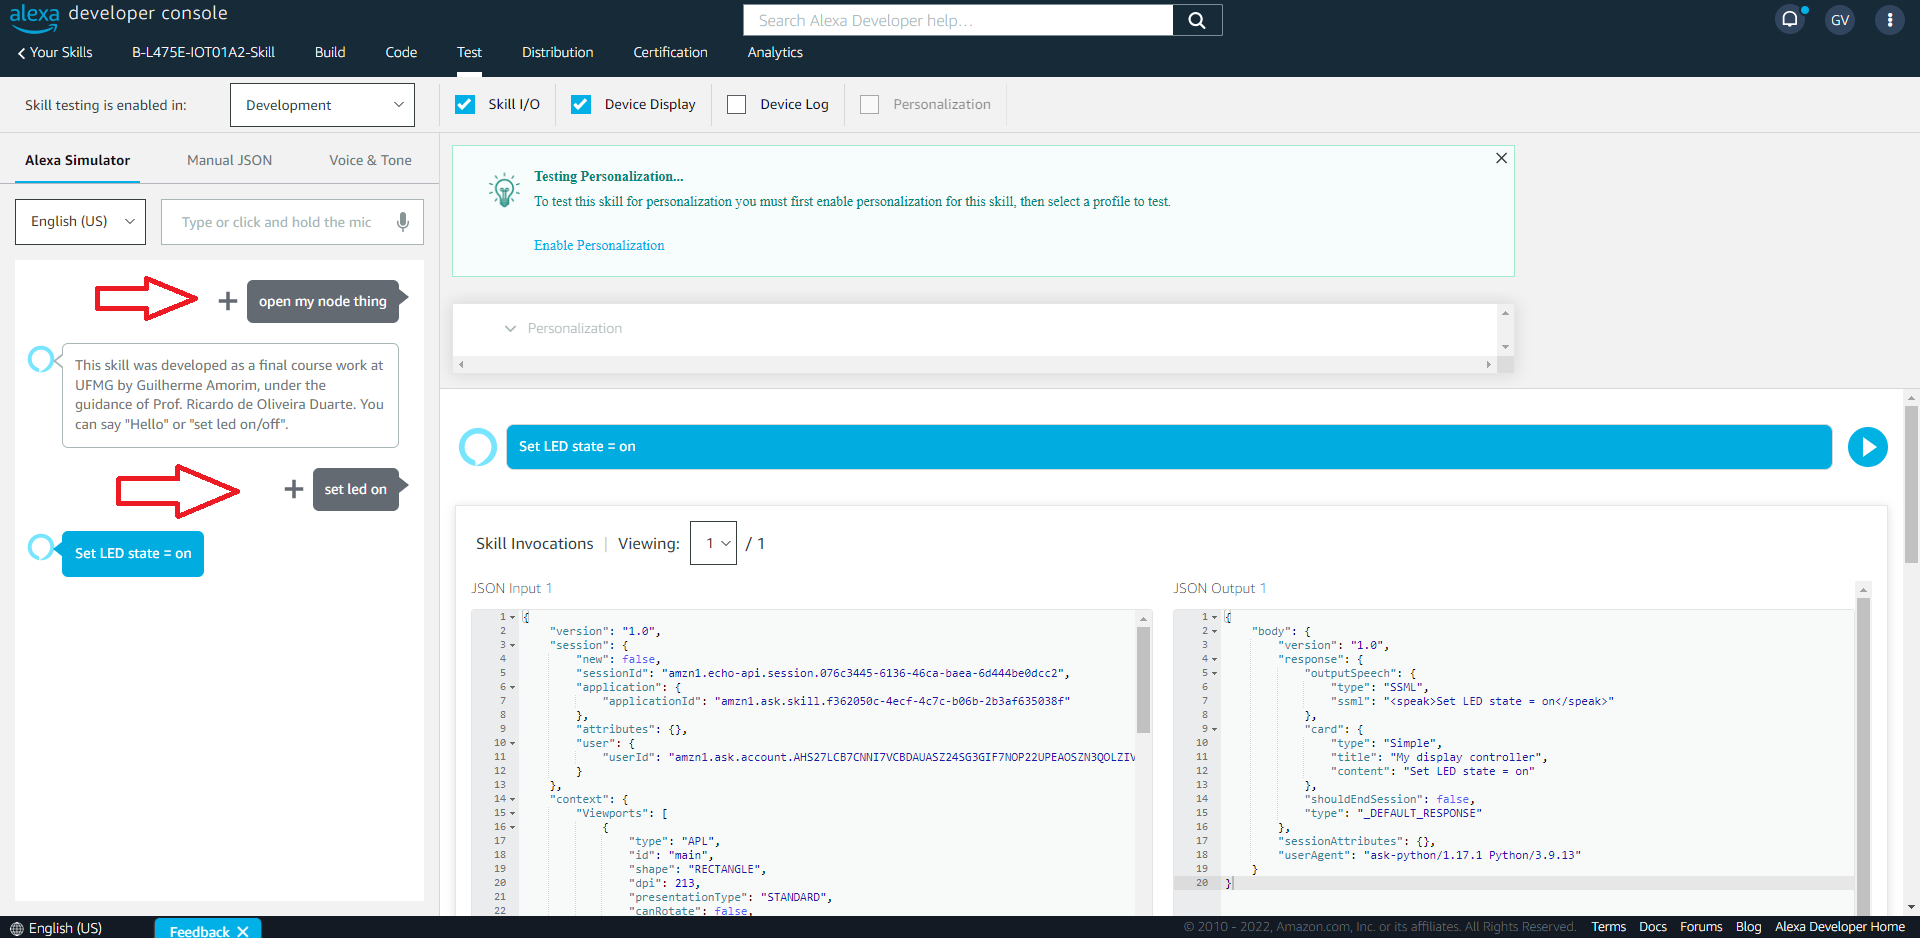
\includegraphics[scale=0.315]{Imagens/alexa_developer_console.png}
	\legend{Fonte: Produzido pelo autor (2022).}
	\label{fig:alexa_developer_console}
\end{figure}

\begin{figure}[htbp]
	\centering
	\caption{Cliente de teste MQTT durante a execução da habilidade \textit{B-L475E-IOT01A2-Skill}.}
	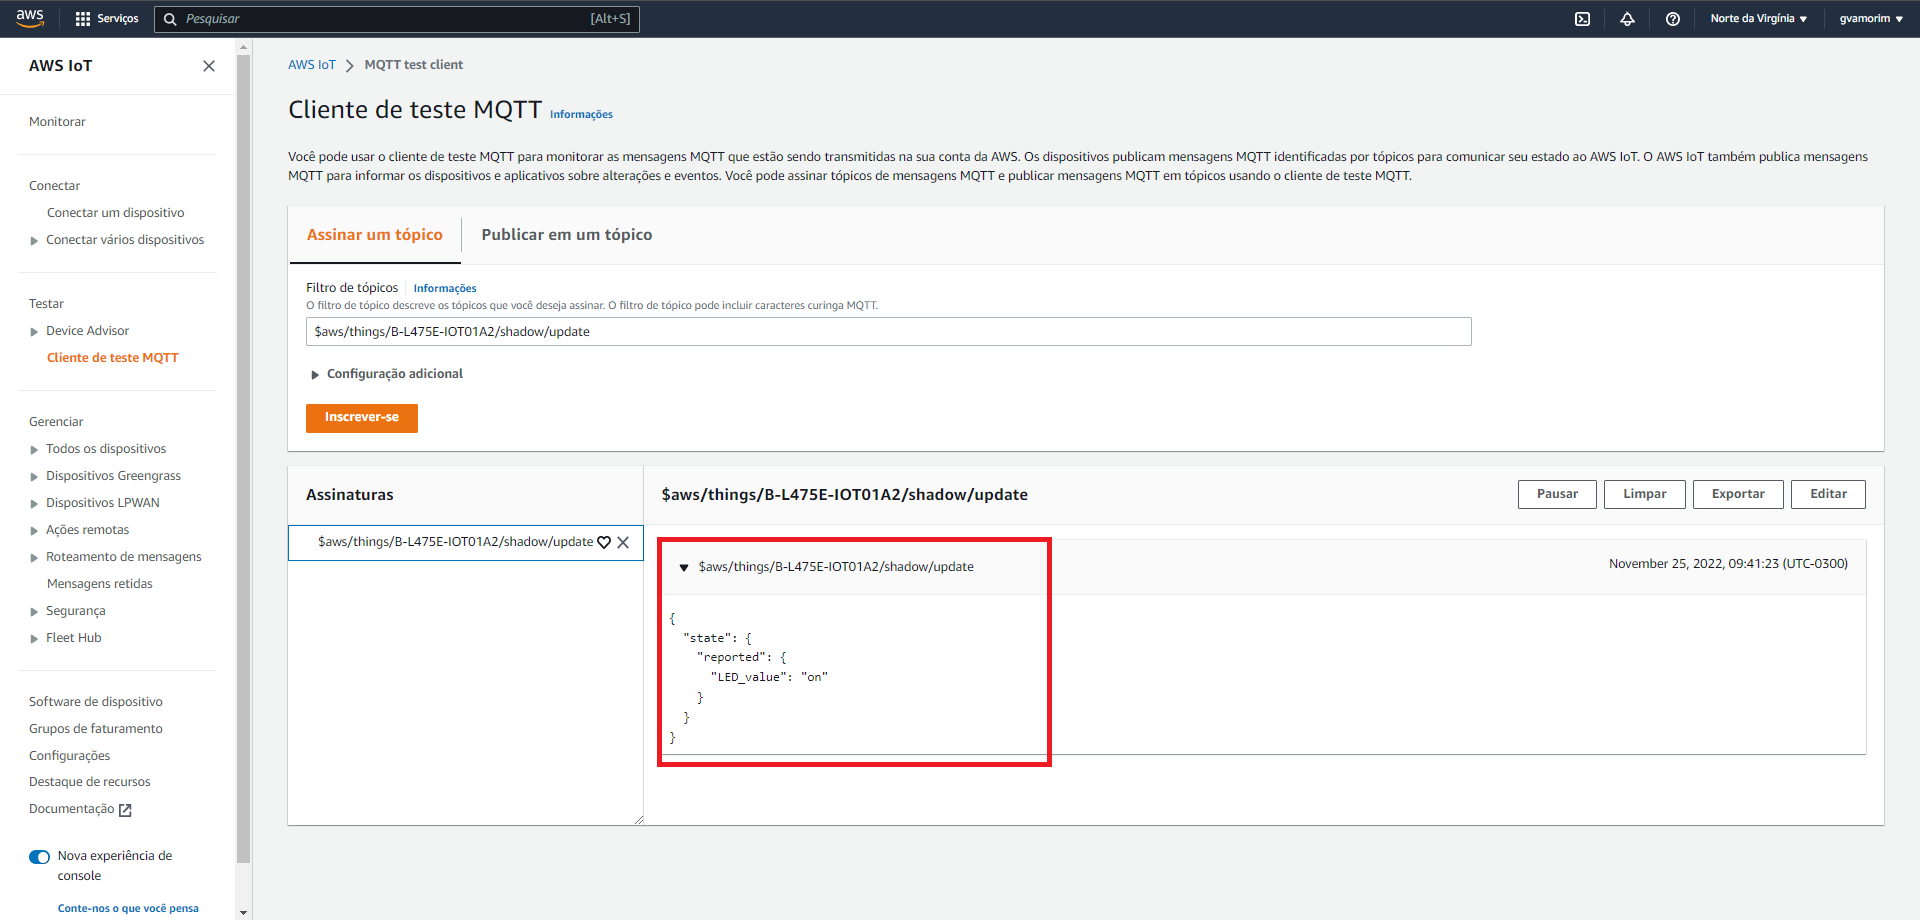
\includegraphics[scale=0.315]{Imagens/cliente_de_teste_mqtt.png}
	\legend{Fonte: Produzido pelo autor (2022).}
	\label{fig:cliente_de_teste_mqtt}
\end{figure}

Para os testes com o dispositivo \textit{B-L475E-IOT01A2}, também utilizou-se o \textit{Cliente de teste MQTT}. O primeiro passo foi a configuração do dispositivo via USB, processo detalhado na \autoref{section:configuracao_dispositivo_bl475eiot01a2_via_usb}. Durante a execução da aplicação, dois tipos de mensagens são enviadas para o tópico MQTT ``\$aws/things/B-L475E-IOT01A2/shadow/update'': uma com com os dados atualizados dos sensores do kit de desenvolvimento e outra com uma requisição de alteração do estado do LED caso o botão da placa seja acionado. As figuras \autoref{fig:cliente_de_teste_mqtt_sensores} e \autoref{fig:cliente_de_teste_mqtt_led_state} mostram capturas de tela do \textit{Cliente de teste MQTT} ao receber mensagens de atualização de dados dos sensores e de requisição de alteração do estado do LED, respectivamente.

\begin{figure}[htbp]
	\centering
	\caption{Mensagem de atualização os dados dos sensores do protótipo recebidos no Cliente de teste MQTT.}
	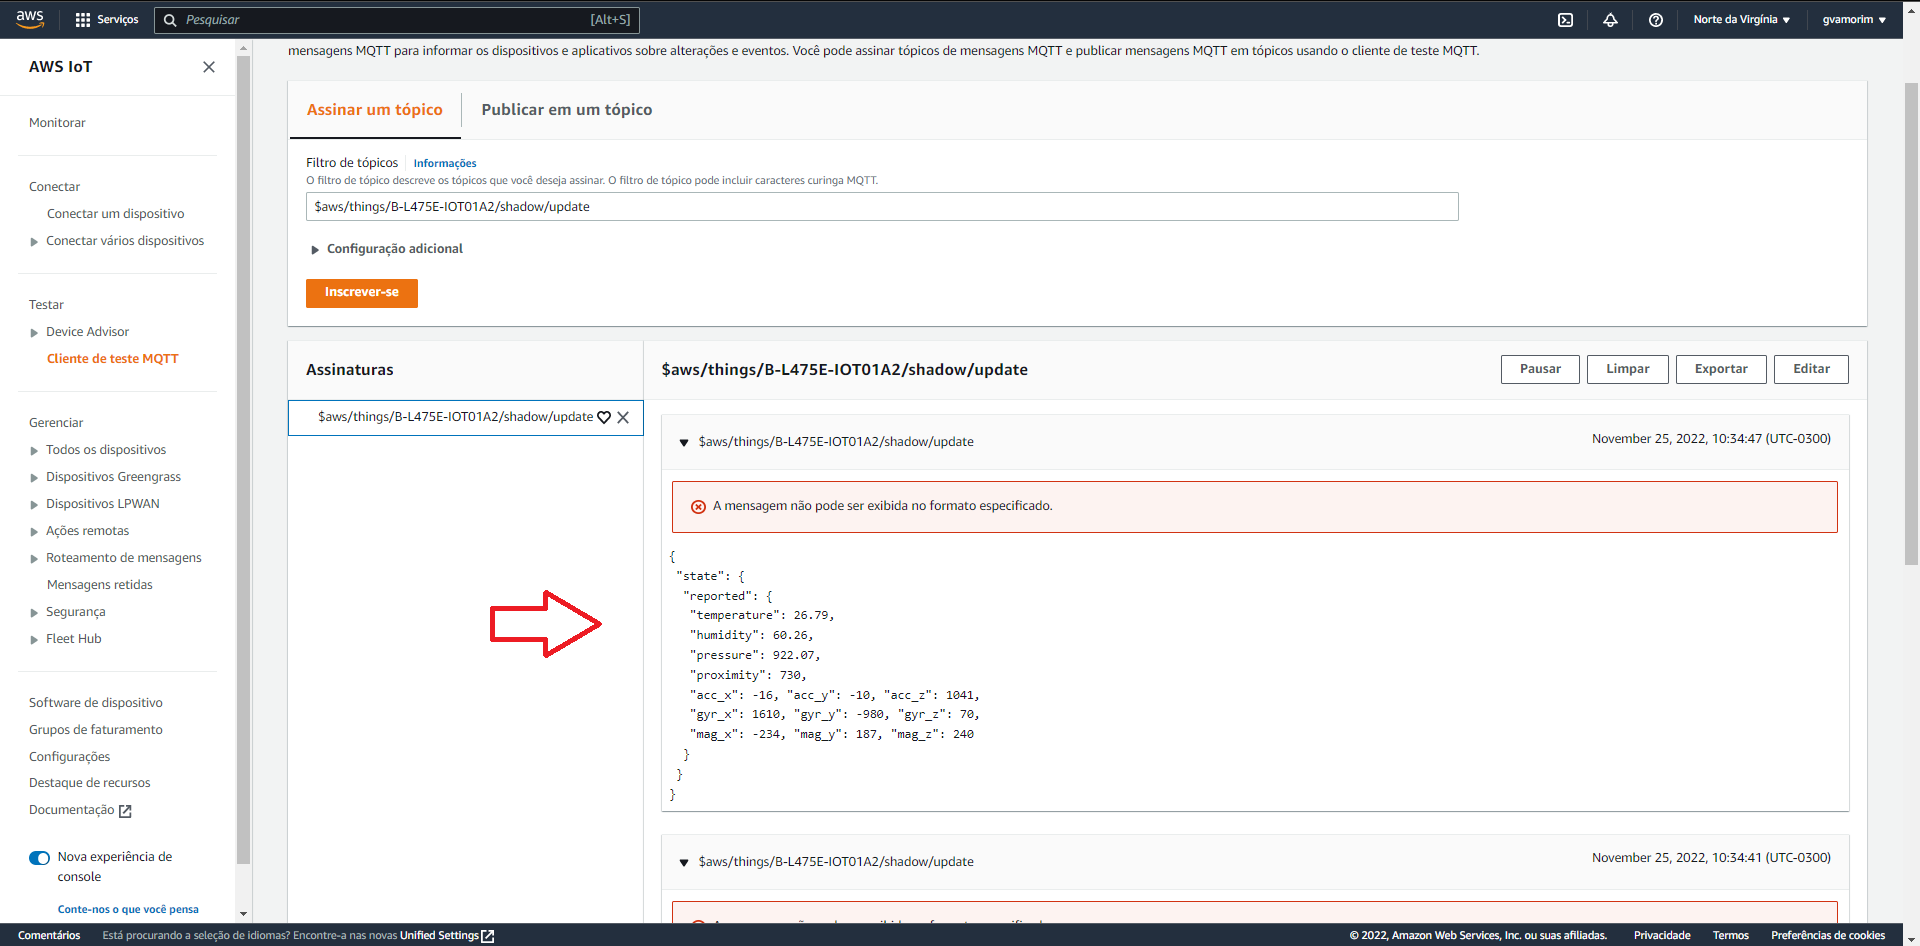
\includegraphics[scale=0.315]{Imagens/cliente_de_teste_mqtt_sensores.png}
	\legend{Fonte: Produzido pelo autor (2022).}
	\label{fig:cliente_de_teste_mqtt_sensores}
\end{figure}

\begin{figure}[htbp]
	\centering
	\caption{Mensagem de requisição de alteração do estado do LED do protótipo recebidos no Cliente de teste MQTT.}
	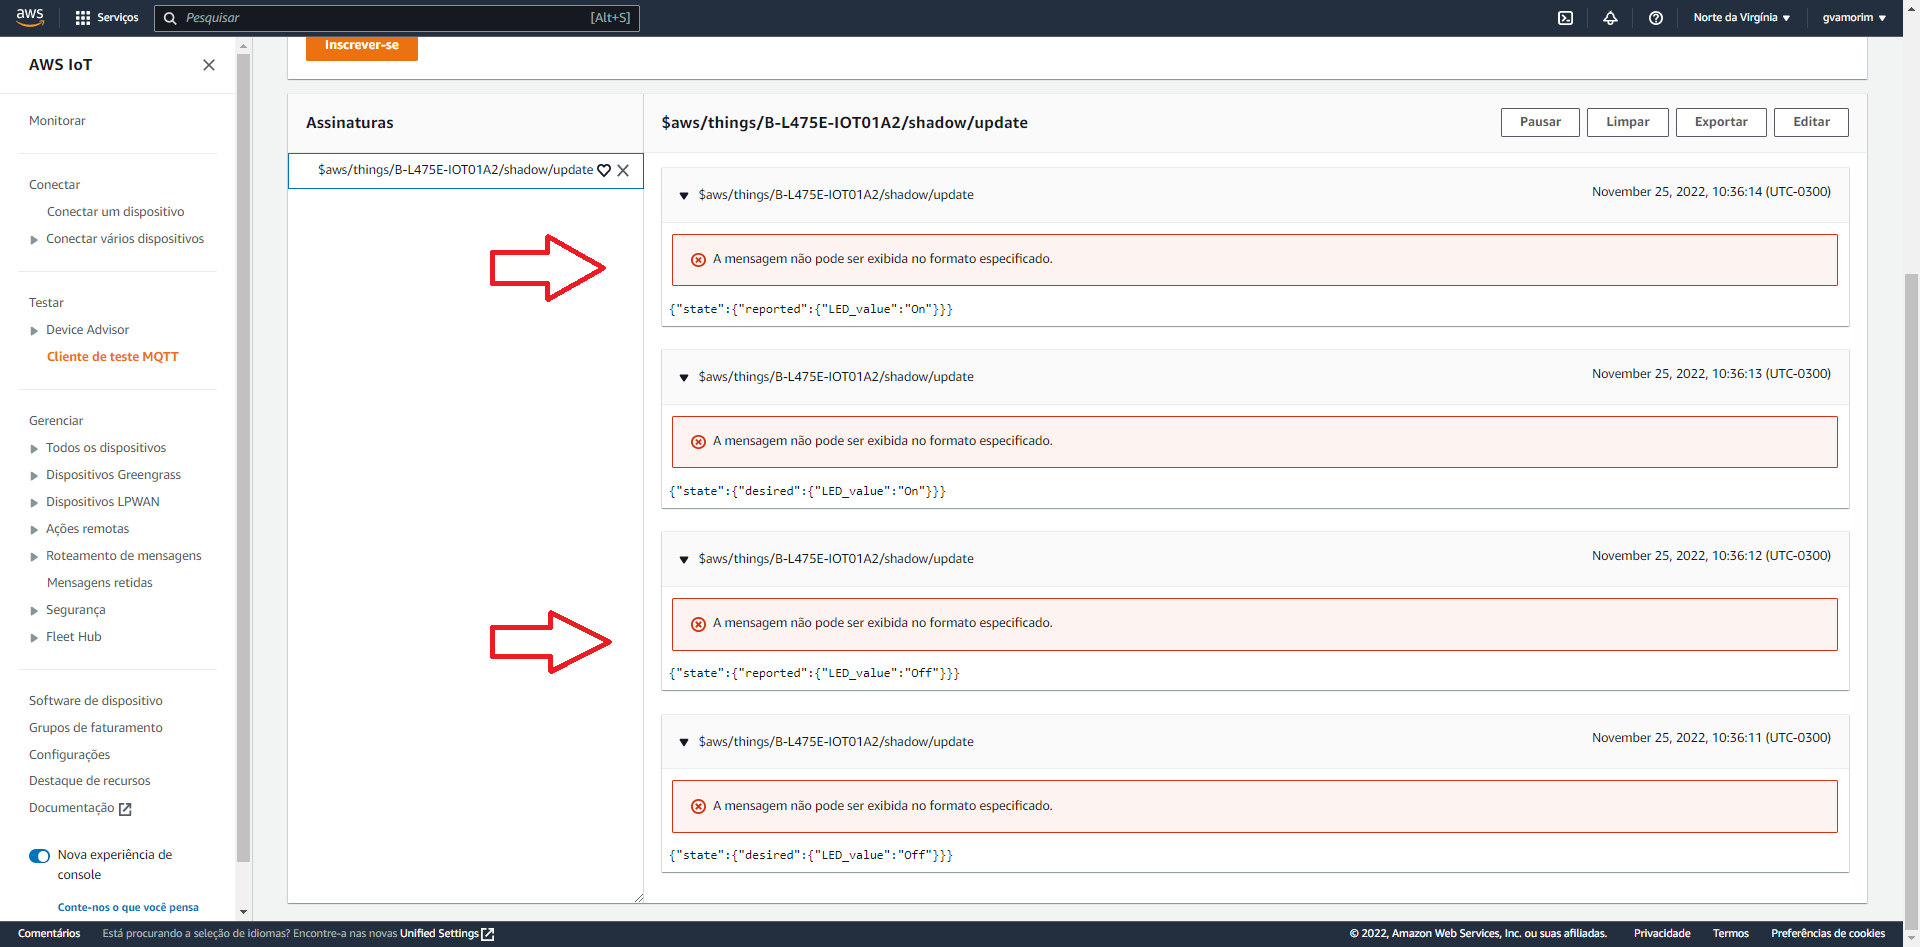
\includegraphics[scale=0.315]{Imagens/cliente_de_teste_mqtt_led_state.png}
	\legend{Fonte: Produzido pelo autor (2022).}
	\label{fig:cliente_de_teste_mqtt_led_state}
\end{figure}

Após os testes individuais do dispositivo \textit{B-L475E-IOT01A2} e da habilidade \textit{B-L475E-IOT01A2-Skill}, testou-se a alteração do estado do LED no dispositivo após o pronunciamento ``set led on'' para a Alexa. O vídeo \href{https://github.com/guiguitz}{PENDING} mostra a execução completa do teste.
